% ============================================================
% Lecture 16 -- Interval estimates and hypothesis tests for coefficients
% ============================================================
\section{Interval Estimates and Hypothesis Tests for the Coefficients}\label{sec:L16}

\lectureheader{16}{dXYKDrO7vE8}{Week-5 R code \texttt{Feb21.r} (Boston lab: \texttt{summary}, \texttt{confint}; $t$-distribution functions \texttt{pt}, \texttt{qt}). The Week-5 lecture PDF was \emph{not} accessed. The theory is filled in from the course's own framework.}

\begin{guiding*}
By the end of this lecture you should be able to:
\begin{itemize}
  \item show that $\RSS/(n-r)$ is an unbiased estimate of $\sigma^2$;
  \item under normal errors, derive the distribution of $(\hat\beta_j-\beta_j)/\widehat{\mathrm{SE}}(\hat\beta_j)$;
  \item construct confidence intervals for regression coefficients and test $H_0:\beta_j=0$;
  \item read the coefficient table of \texttt{summary(lm(...))}.
\end{itemize}
\end{guiding*}

\subsection{Recap}
$\hat\beta$ is unbiased with $\Cov\hat\beta=\sigma^2(X\T X)^{-1}$ (\cref{thm:L15-moments}). To turn this into
confidence intervals and tests we need two more things: an estimate of the unknown $\sigma^2$, and the
exact distribution of the estimates. The latter requires the normality assumption, which also
underlies \cref{thm:L08-dist}.

\subsection{Estimating $\sigma^2$}
\begin{theorem}\label{thm:L16-s2}
In the linear model $(Y,X\beta,\sigma^2I_n)$ with $\rank X=r<n$, the residual sum of squares
$\RSS=\pnorm{Y-X\hat\beta}^2=\pnorm{(I-\PX)Y}^2$ satisfies $\EE[\RSS]=(n-r)\sigma^2$. Hence
\[
s^2=\frac{\RSS}{n-r}
\]
is an unbiased estimate of $\sigma^2$.
\end{theorem}
\begin{proof}
Let $M=I-\PX$. It is symmetric and idempotent (\cref{prob:L14-1}), so $\RSS=Y\T M\T MY=Y\T MY$. Since
$MX=X-\PX X=0$ (every column of $X$ lies in $\colsp{X}$), we get $MY=M(X\beta+\eps)=M\eps$ and $\RSS=\eps\T M\eps$. For any fixed matrix $M$,
\[
\EE[\eps\T M\eps]=\EE\Bigl[\sum_{i,l}M_{il}\eps_i\eps_l\Bigr]=\sum_{i,l}M_{il}\,\sigma^2\mathbbm 1\{i=l\}=\sigma^2\tr M ,
\]
using $\EE[\eps_i\eps_l]=\sigma^2$ if $i=l$ and $0$ otherwise. Finally
$\tr M=n-\tr\PX=n-r$ (\cref{lem:L14-projection}).
\end{proof}
In simple linear regression $r=2$ and $s^2=\RSS/(n-2)$. Its square root is the \emph{residual standard
error} of \cref{sec:L17}. For the one-way model $r=k$ and $s^2=\SSW/(n-k)$ (\cref{prob:L08-1}).

\subsection{Distributions under normality}
\begin{theorem}[Sampling distribution of $\hat\beta$]\label{thm:L16-dist}
Assume $\eps\sim\N(0,\sigma^2I_n)$ and $\rank X=p<n$. Then
\begin{enumerate}
  \item $\hat\beta\sim\N\bigl(\beta,\sigma^2(X\T X)^{-1}\bigr)$;
  \item $\RSS/\sigma^2\sim\chi^2_{n-p}$;
  \item $\hat\beta$ and $\RSS$ are independent;
  \item for each $j$, with $v_{jj}=[(X\T X)^{-1}]_{jj}$ and $\widehat{\mathrm{SE}}(\hat\beta_j)=s\sqrt{v_{jj}}$,
  \[
  T_j=\frac{\hat\beta_j-\beta_j}{\widehat{\mathrm{SE}}(\hat\beta_j)}\sim t_{n-p}.
  \]
\end{enumerate}
\end{theorem}
\begin{proof}
(1) $\hat\beta=(X\T X)^{-1}X\T Y$ is a linear function of the normal vector $Y$, so it is normal. Its mean and
covariance are given by \cref{thm:L15-moments}.
(2) As in the proof of \cref{thm:L16-s2}, $\RSS/\sigma^2=Z\T MZ$ with $Z=\eps/\sigma\sim\N(0,I_n)$ and $M=I-\PX$
symmetric idempotent of rank $n-p$. \Cref{lem:L08-chisq} gives $\chi^2_{n-p}$.
(3) $\hat\beta$ is a function of $U=X\T Y$, and $\RSS=\pnorm{MY}^2$ is a function of $V=MY$. The pair $(U,V)$ is jointly normal,
and $\Cov(X\T Y,MY)=X\T(\sigma^2I)M\T=\sigma^2(MX)\T=0$. By \cref{lem:L08-indep}, $U\indep V$, so $\hat\beta\indep\RSS$.
(4) $Z_j=(\hat\beta_j-\beta_j)/(\sigma\sqrt{v_{jj}})\sim\N(0,1)$ by (1). Also $W=\RSS/\sigma^2\sim\chi^2_{n-p}$ by (2), and $Z_j\indep W$ by (3).
Then $T_j=Z_j/\sqrt{W/(n-p)}$, which is the definition of the $t_{n-p}$ distribution. The unknown $\sigma$ cancels.
\end{proof}

\begin{corollary}[Confidence interval and $t$-test]\label{cor:L16-ci}
Let $t_{n-p,\,1-\alpha/2}$ be the $(1-\alpha/2)$-quantile of $t_{n-p}$ (R: \texttt{qt(1-alpha/2, df)}).
\begin{enumerate}
  \item $\hat\beta_j\pm t_{n-p,\,1-\alpha/2}\,\widehat{\mathrm{SE}}(\hat\beta_j)$ is a $100(1-\alpha)\%$ confidence interval for $\beta_j$.
  \item To test $H_0:\beta_j=b$ against $H_1:\beta_j\ne b$, use $t=(\hat\beta_j-b)/\widehat{\mathrm{SE}}(\hat\beta_j)$. Reject at level $\alpha$ if $\abs t>t_{n-p,1-\alpha/2}$. The p-value is $2\,\PP(T>\abs t)$ for $T\sim t_{n-p}$ (R: \texttt{2*(1-pt(abs(t), df))}).
\end{enumerate}
\end{corollary}
\begin{proof}
(1) $\PP\bigl(\abs{T_j}\le t_{n-p,1-\alpha/2}\bigr)=1-\alpha$ by symmetry of the $t$ distribution. Rearranging the inequality
$\abs{\hat\beta_j-\beta_j}\le t_{n-p,1-\alpha/2}\widehat{\mathrm{SE}}$ gives the interval.
(2) Under $H_0$, $t\sim t_{n-p}$, so $\PP_{H_0}(\abs t>t_{n-p,1-\alpha/2})=\alpha$.
\end{proof}

\begin{example}[By hand: the four-point data]\label{ex:L16-hand}
$x=(1,2,3,4)$, $Y=(2,3,5,6)$, with $\hat\beta=(0.5,1.4)$ and $\RSS=0.2$ (\cref{ex:L05-hand}). Here $n-p=2$.
\begin{itemize}
  \item $s^2=0.2/2=0.1$ and $s=0.3162$.
  \item $\widehat{\mathrm{SE}}(\hat\beta_1)=\sqrt{0.1\times 0.2}=\sqrt{0.02}=0.14142$ and $\widehat{\mathrm{SE}}(\hat\beta_0)=\sqrt{0.1\times1.5}=0.38730$ (\cref{ex:L15-hand}).
  \item $t$ for $H_0:\beta_1=0$: $1.4/0.14142=9.8995$. With $2$ degrees of freedom the p-value is $2\PP(T>9.8995)=0.01005$, so we reject at $5\%$ but not at $1\%$.
  \item $t_{2,0.975}=4.3027$. The $95\%$ interval for $\beta_1$ is $1.4\pm4.3027\times0.14142=1.4\pm0.6085=(0.7915,\,2.0085)$.
  \item Intercept: $t=0.5/0.3873=1.291$ with p-value $0.326$. Its $95\%$ interval is $0.5\pm1.6664=(-1.1664,\,2.1664)$, which contains $0$.
\end{itemize}
With only $2$ degrees of freedom, the quantile $4.30$ is far larger than the normal $1.96$.
\end{example}

\subsection{The Boston example from the R code}
\begin{example}[\texttt{medv} on \texttt{lstat}]\label{ex:L16-boston}
The code follows the lab of Chapter~3 of \emph{An Introduction to Statistical Learning}. \texttt{Boston} has
$n=506$ census tracts. \texttt{medv} is the median house value (in \$1000s), and \texttt{lstat} is the
percentage of lower-status population. The first call, \texttt{lm(medv \textasciitilde\ lstat)}, gives an error
because \texttt{Boston} was not specified as the data. The fix is \texttt{data = Boston}, or \texttt{attach(Boston)}.
\texttt{summary(lm.fit)} prints
\begin{center}
\begin{tabular}{lrrrr}\hline
 & Estimate & Std.\ Error & $t$ value & $\PP(>\abs t)$\\\hline
(Intercept) & $34.5538$ & $0.5626$ & $61.415$ & $<2\times10^{-16}$\\
lstat & $-0.9500$ & $0.0387$ & $-24.528$ & $<2\times10^{-16}$\\\hline
\end{tabular}
\end{center}
on $504$ degrees of freedom. \texttt{confint(lm.fit)} gives the $95\%$ intervals
\[
\beta_0\in(33.4485,\ 35.6592),\qquad \beta_1\in(-1.0261,\ -0.8740),
\]
i.e.\ $\hat\beta_j\pm1.9647\,\widehat{\mathrm{SE}}$, where $t_{504,0.975}=1.9647$. Each additional percentage point of
lower-status population is associated with a decrease of between \$874 and \$1026 in median value. The
relationship is overwhelmingly significant. (The residual plot in \cref{sec:L18} shows that it is also
not linear.)
\end{example}

\subsection{The $t$ distribution in R}
The last part of the R code explores the $t$ distribution.
\begin{itemize}
  \item \texttt{1 - pt(1:5, df = 1)} gives the upper-tail probabilities $0.25000, 0.14758, 0.10242, 0.07798, 0.06283$. The Cauchy ($t_1$) tails are very heavy.
  \item \texttt{qt(.975, df = c(1:10,20,50,100,1000))} gives $12.706, 4.303, 3.182, 2.776, 2.571,\dots,2.228$ ($df=10$), $2.086$ ($20$), $2.009$ ($50$), $1.984$ ($100$) and $1.962$ ($1000$). As the degrees of freedom grow, the quantiles decrease to the normal value $1.960$.
  \item The non-central $t$ distribution (\texttt{pt(t, df=3, ncp=d)}, drawn with \texttt{image}/\texttt{persp}) is the distribution of $T_j$ when $H_0$ is \emph{false}. It determines the power of the $t$-test.
\end{itemize}

\begin{figure}[ht]
\centering
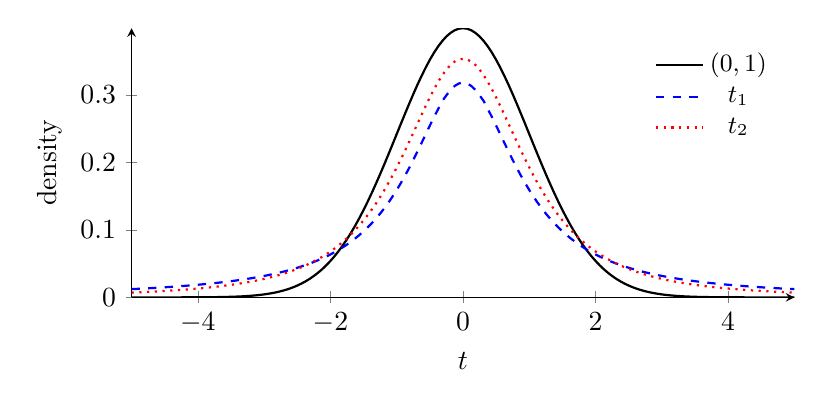
\begin{tikzpicture}
\begin{axis}[width=10cm,height=5cm,domain=-5:5,samples=161,axis lines=left,xlabel={$t$},ylabel={density},
  legend style={font=\small,draw=none,at={(0.98,0.95)},anchor=north east}]
\addplot[thick,black] {exp(-x^2/2)/sqrt(2*pi)};
\addplot[thick,blue,dashed] {1/(pi*(1+x^2))};
\addplot[thick,red,dotted] {0.3536*(1+x^2/2)^(-1.5)};
\legend{{$\N(0,1)$},{$t_1$},{$t_2$}}
\end{axis}
\end{tikzpicture}
\caption{The $t$ densities have heavier tails than the normal. This is why the critical values exceed $1.96$ when the degrees of freedom are small.}
\label{fig:L16-t}
\end{figure}

\subsection{Computation}
\begin{center}\small
\begin{tabular}{@{}>{\raggedright\arraybackslash}p{6.5cm}>{\raggedright\arraybackslash}p{8.9cm}@{}}\hline
R & Python\\\hline
\texttt{summary(lm.fit)} & \texttt{fit.summary()} (or \texttt{fit.params}, \texttt{fit.bse}, \texttt{fit.tvalues}, \texttt{fit.pvalues})\\
\texttt{confint(lm.fit)} & \texttt{fit.conf\_int()}\\
\texttt{pt(q, df)}, \texttt{qt(p, df)} & \texttt{scipy.stats.t.cdf(q, df)}, \texttt{stats.t.ppf(p, df)}\\
\texttt{pt(t, df, ncp)} & \texttt{stats.nct.cdf(t, df, ncp)}\\\hline
\end{tabular}
\end{center}
\nb{week05/L16\_intervals\_tests.ipynb} computes the coefficient table from the formulas, checks it against
\texttt{statsmodels}, and verifies the $95\%$ coverage and the $t_{n-p}$ distribution by simulation.

\subsection{Summary}
\begin{itemize}
  \item $s^2=\RSS/(n-r)$ is unbiased for $\sigma^2$, because $\EE[\eps\T M\eps]=\sigma^2\tr M$.
  \item Under normality: $\hat\beta\sim\N(\beta,\sigma^2(X\T X)^{-1})$, $\RSS/\sigma^2\sim\chi^2_{n-p}$, and they are independent. So $(\hat\beta_j-\beta_j)/\widehat{\mathrm{SE}}\sim t_{n-p}$.
  \item CI: $\hat\beta_j\pm t_{n-p,1-\alpha/2}\widehat{\mathrm{SE}}$. Test of $\beta_j=0$: $t=\hat\beta_j/\widehat{\mathrm{SE}}$.
  \item Boston: $\hat\beta_1=-0.9500$ (SE $0.0387$), CI $(-1.0261,-0.8740)$.
\end{itemize}

\subsection{Exercises}
\begin{problem}\label{prob:L16-1}
For the snowfall data of \cref{ex:L07-snow}, test $H_0:\beta_1=0$ at the $5\%$ level and give a $95\%$ CI for the slope.
\end{problem}
\begin{problem}\label{prob:L16-2}
Show that in simple linear regression the $t$ statistic for $\beta_1=0$ can be written $t=r\sqrt{n-2}/\sqrt{1-r^2}$, where $r$ is the sample correlation.
\end{problem}
\begin{problem}\label{prob:L16-3}
Why can we not use $\RSS/n$ in place of $s^2$ in \cref{thm:L16-dist}(4)? What is $\EE[\RSS/n]$?
\end{problem}
\begin{problem}\label{prob:L16-4}
In \cref{ex:L16-hand}, test $H_0:\beta_1=1$ against $\beta_1\ne 1$ at the $5\%$ level.
\end{problem}
\begin{problem}\label{prob:L16-5}
Simulate $10\,000$ data sets from $Y_i=0.5+1.4x_i+\eps_i$, $\eps_i\sim\N(0,0.1)$, $x=(1,2,3,4)$, and estimate the coverage of the $95\%$ interval for $\beta_1$.
\end{problem}

\subsection{Further reading}
Christensen, \S2.6 (sampling distributions), Chapter~3 (testing) and Chapter~6; Rao, \S4b (tests of linear
hypotheses); ISLR \S3.1.2.
